\namedchapter{Projektmanagement}{K}
Für die Umsetzung eines Projektes ist ein Team bestehend aus Mitgliedern, welche bestenfalls unterschiedliche Kernkompetenzen haben, erforderlich. Damit ein Projekt am Ende auch einen guten Abschluss findet, sollte zu Beginn ein Vorgehensmodell festgelegt und ein grober Zeitplan erstellt werden. Aus diesen Gründen werden die konkrete Vorgehensweise nach SCRUM, die Rollen- und Aufgabenverteilung und der Zeitplan nachfolgend beschrieben. Abschließend werden in diesem Kapitel die verwendeten Tools und ihr Einsatz im Projekt dargestellt.
\section{SCRUM}
Im Folgenden wird die Entscheidung für ein agiles Vorgehensmodell begründet sowie die genaue Rollen-und Aufgabenverteilung dargestellt.

\subsection{Agiles Vorgehen}
Prozessmodelle legen den organisatorischen Rahmen für eine Entwicklung fest indem sie unter anderem den Arbeitsablauf, die dabei durchzuführenden Aktivitäten sowie die Verantwortlichkeiten und Kompetenzen im Team festlegen. \cite{amberg2011wertschopfungsorientierte} Prozessmodelle ermöglichen damit eine kontrollierte und disziplinierte Entwicklung. \cite{amberg2011wertschopfungsorientierte} Zu Beginn des Projektes wurden grundlegende Prozessmodelle, wie zum Beispiel das Wasserfallmodell ausgeschlossen, da diese insbesondere für das vorliegende Projekt einige Nachteile aufweisen. Häufig können bei dieser Art von Prozessmodellen Risikofaktoren weniger berücksichtigt werden. Zudem ist das sequentielle vollständige Durchlaufen einer Projektphase für das vorliegende Projekt nicht immer sinnvoll. \cite{amberg2011wertschopfungsorientierte} Code-getriebene Modelle, wie beispielsweise das evolutionäre Modell, hemmen den Entwicklungsprozess und mögliche Wege durch festgelegte Zwischenergebnisse. \cite{amberg2011wertschopfungsorientierte, balzert2000lehrbuch} Agile Entwicklungsmodelle wie Scrum setzen auf die Selbstorganisation der einzelnen Teammitglieder. \cite{scrum} Durch Festlegung von Meetings, Artefakten und Rollen bietet das Modell einen groben Rahmen, lässt aber genug Freiraum, um Anforderungen immer wieder kontinuierlich an die Gegebenheiten und die Kundenwünsche anzupassen.
Aufgrund der zuvor genannten Aspekte, der Teamgröße und der Entwicklung eines Produktes, welches genau den Anforderungen von Statistance entsprechen soll, wurde Scrum als agiles Vorgehensmodell gewählt. Durch regelmäßige Rücksprachen und das demonstrieren verschiedener Prototypen konnten die Anforderungen kontinuierlich angepasst werden. Zum Projektstart wurden zweiwöchige Sprints festgelegt. Eine Ausnahme stellt der erste Sprint dar, welcher eine Woche umfasste. In der ersten Woche wurden insbesondere organisatorische Aufgaben abgewickelt. Zweimal wöchentlich gab es Meetings vor Ort und via Skype. Die Sprint Planning Meetings fanden zu Beginn eines Sprints statt. Bei den Meetings wurden Inhalte des nächsten Sprints festgelegt und dokumentiert. Hierbei wurden Priorität und Aufwand der Aufgaben mit einbezogen. Aufgaben aus dem Product Backlog wurden ausgewählt und entsprechenden Teammitgliedern zugewiesen. Mit der Festlegung der Aufgaben wurde ebenfalls ein Sprintziel definiert. Rücksprachen mit Statistance fanden regelmäßig ca. alle zwei Wochen statt. Zwischen den Treffen vor Ort gab es zudem regelmäßige Rücksprachen über Kommunikations-Tools, welche in Abschnitt \ref{subsubsec:kommunikation} beschrieben werden. Daily Scrum Meetings wurden nicht abgehalten, jedoch regelmäßig Updates während eines Sprints durch einzelne Teammitglieder gegeben beziehungsweise eingeholt. Das wöchentliche Skype-Meeting diente als eine Art Sprint Review Meeting beziehungsweise Retrospektive. Die erzielten (Zwischen-) Ergebnisse wurden nacheinander besprochen. Jeder Teilnehmer des Meetings konnte seine (Zwischen-) Ergebnisse präsentieren und Feedback zu anderen geben. Zukünftige Verbesserungen und die Weiterentwicklung wurden ebenfalls besprochen. Durch das Einholen von Feedback durch Statistance konnten neue Anforderungen nach jeder Iteration in den nächsten Sprint einfließen. Ab der Entwicklungsphase ging aus jedem Sprint ein lauffähiges Produkt hervor, welches sich immer mehr dem reinen Endprodukt annäherte. 


\subsection{Rollen- und Aufgabenverteilung}
An dem \textit{Praxisprojekt Anwendungssysteme} haben insgesamt sechs Personen mitgewirkt. Die Mitglieder studieren im Bachelor oder Master Wirtschaftsinformatik beziehungsweise Information Systems Management oder Informatik. Es vereinen sich daher unter anderem Kompetenzen aus den Bereichen Frontend- und Backendentwicklung sowie Projektmanagement. Jedes Mitglied konnte seine Kompetenzen bei entsprechenden Aufgaben gut einbringen, die eigene Kompetenzen ausbauen und neue dazu gewinnen.
Die einzelnen Aufgaben jedes Teammitglieds sind in Tabelle \ref{tab:tasks} dargestellt.
\begin{table}[h!]
\begin{tabular}{|p{7cm}|c|c|c|c|c|c|}
\hline
\textbf{A} & \textbf{F}  & \textbf{J} & \textbf{J}& \textbf{T} & \textbf{M} & \textbf{K} \\ \hline \bottomrule
Projektmanagement und \newline Architekturüberblick &  &  &  & X &  & X \\ \hline
Recherche & X & X & X & X & X & X \\ \hline
Batch-Jobs &  &  &  & X &  &  \\ \hline
Sage 100 Integration &  & X & X &  &  &  \\ \hline
API & X &  & X & X &  & X \\ \hline
Spring Security &  &  &  & & X &  \\ \hline
Frontend  & X &  & X &  &  &  \\ \hline
Config Management  &  & X &  & X & X &  \\ \hline
API Gateway &  & X &  &  & X & X \\ \hline
\end{tabular}
\caption{Aufgabenverteilung}
\label{tab:tasks}
\end{table}

Für die Kommunikation mit Statistance und M. wurde ein Projektleiter festgelegt. Der Projektleiter hatte zudem die Aufgabe, dass Abgaben (zum Beispiel Zwischenpräsentationen) fristgerecht fertiggestellt und abgegeben werden. Eine weitere Person im Team hatte die Aufgabe die technische Umsetzung der Architektur im Blick zu behalten, damit alle notwendigen technischen Aufgaben richtig und fristgerecht umgesetzt werden. An der Entwicklung waren alle sechs Teammitglieder beteiligt, sodass sich das Entwicklungsteam aus allen sechs Teammitgliedern zusammensetzte.
\section{Zeitplan und Meilensteine}

In der Vorplanungsphase wurden organisatorische Aufgaben abgearbeitet. Diese umfassten die Organisation im Team, wie beispielsweise die Rollenverteilung sowie die konkrete Anforderungsanalyse durch Gespräche mit Statistance. Auch Entwicklungswerkzeuge wurden in der ersten Woche festgelegt. Von Ende Oktober bis Mitte November gab es eine intensive Recherchephase. In dieser Phase wurden verschiedenste Frameworks, Programmiersprachen, Datenbankmodelle und mögliche Architekturen analysiert und auf ihre Eignung hinsichtlich des Projektes evaluiert. In dem darauffolgenden Sprint wurde insbesondere Open Integration Hub als mögliches Framework zur Umsetzung der Aufgabe analysiert und eine Kostenkalkulation aufgestellt. Mögliche Umsetzungsoptionen wurden Statistance präsentiert. Eine konkrete Entscheidungsfindung gab es im Dezember 2019. Hierbei wurde die finale Architektur festgelegt sowie die Designs des Domänenmodells und des Daten-Mappings. Im gleichen Monat begann zusätzlich die konkrete Implementierung des zu entwickelnden Architekturmodells. Eine Zwischenpräsentation lieferte einen Überblick über das bis dato Geschehene. Während im Dezember 2019 zunächst die Integration von Sage 100 fokussiert wurde, kamen im Januar 2020 die Umsetzung der API, Spring Security und die Implementierung der Batch-Jobs hinzu. Abschließend wurden im Februar 2020 ein Frontend zur Steuerung der Batch-Jobs und das API Gateway implementiert sowie das Config Management realisiert. Insgesamt gab es drei Prototypen. Die ersten zwei Prototypen waren statisch. Batchjobs wurden im gleichen Turnus ausgeführt. Der dritte Prototyp ist dynamisch, da eine individuelle Ausführung verschiedener Batch-Jobs ermöglicht wird. Der dritte Prototyp stellt zugleich das Endprodukt dar. Tabelle \ref{tab:sprints} bietet einen Überblick über die einzelnen Sprints mit dem entsprechenden Zeitraum als auch über die Kernaufgaben des Sprints. Die zu Beginn und auch im Laufe des Projektes immer wieder angepassten Aufgaben konnten im festgelegten Zeitraum umgesetzt werden. Den Abschluss des Projektes stellte die Abschlusspräsentation am 10. Februar 2020 dar. 

\begin{table}[h!]
\begin{tabular}{|c|c|p{7cm}|c|}
\hline
\textbf{Sprint} & \textbf{Zeitraum} & \textbf{Aufgaben} &  \textbf{Prototyp}\\ \hline \bottomrule
1 & Oktober 2019  & Treffen mit Statistance, Besprechung der konkreten Aufgabe, Team-Organisation &  \\ \hline
2 & Oktober- November 2019  & Recherche (Frameworks, Programmiersprachen, Datenbanken, Schnittstellen zu ERP-Systemen) &  \\ \hline
3 & November - Dezember 2019 & Aufstellung verschiedener Umsetzungsoptionen, Fokus auf Open Integration Hub und Aufstellung der Kostenkalkulation, Anfertigung der Zwischenpräsentation &  \\ \hline
\multicolumn{4}{|c|}{Zwischenpräsentation}   \\ \hline
4 & Dezember 2019 - Januar 2020 & Entscheidung für eine Umsetzungsoption, Design des Domänenmodells und des Mappings der Daten,  Implementierungsstart (Batch-Jobs, Integration Sage 100) & I (statisch) \\ \hline
5 &  Januar 2020 &  Implementierung (Batch-Jobs, API, Spring Security), Set Up auf Testserver von Statistance einrichten & II (statisch) \\ \hline
6 &  Februar 2020 &   Implementierung (Frontend, API Gateway, Config Management), Anfertigung der Abschlusspräsentation & III (dynamisch)  \\
\hline
\multicolumn{4}{|c|}{Abschlusspräsentation}   \\ \hline
\end{tabular}
\caption{Sprints}
\label{tab:sprints}
\end{table}
\newpage

\section{Tools} 
Für das Projekt wurden verschiedene Tools für verschiedene Bereiche verwendet. Diese werden nach ihrer Funktion im Folgenden beschrieben.
\subsection*{\textbf{Kommunikation und Meetings}} \label{subsubsec:kommunikation} 
Kommuniziert wurde primär über den webbasierten Instant-Messaging-Dienst Slack. Verschiedene Channels wurden für verschiedene Aufgabenbereiche erstellt, zum Beispiel für die Implementierung, die Präsentationen und für allgemeine Fragen an andere Teammitglieder. Slack wurde teilweise auch für die Kommunikation mit dem Statistance-Team verwendet. Skype wurde als weiteres Kommunikationstool verwendet. Einmal wöchentlich fand ein Meeting über Skype statt. Besonders die Funktion des Screen-Sharings wurde verwendet, um einen Überblick über die Arbeit anderer Teammitglieder zu gewinnen und eine gemeinsame Sicht zu haben. Aufkommende Fragen im Team wurden gesammelt und entweder mit Statistance persönlich besprochen oder in E-Mails an Statistance gesendet. Besonders für die Kommunikation mit Statistance wurden E-Mails geschrieben. Um individuelle Termine für zusätzliche Meetings, Skype Calls und Rücksprachen mit Statistance zu vereinbaren wurden Umfragen über doodle gemacht. So konnten Termine zeitnahe gefunden werden. Meetings mit Statistance wurden anschließend über E-Mail Kontakt mit dem Unternehmen kommuniziert.

\subsection*{\textbf{Sprint-Planung}}
Für den Sprint-Überblick und den Status der dem Sprint zugeordneten Aufgaben wurde ein Trello-Board verwendet. Die Aufgaben konnten zunächst gesammelt und dann bestimmten Teammitgliedern zugewiesen werden. Durch die verschiedenen Zustände in Progress, Review und Done konnten Teammitglieder den Bearbeitungsstand der eigenen Aufgaben dokumentieren und den von Aufgaben andere Mitglieder gut nachvollziehen. Zudem konnten Informationen beispielsweise zum Setup für andere Teammitglieder festgehalten werden. Ein Zwischenstand vom Trello Board ist in \ref{fig:trello} zu sehen.

\begin{figure}[!h]
\centering
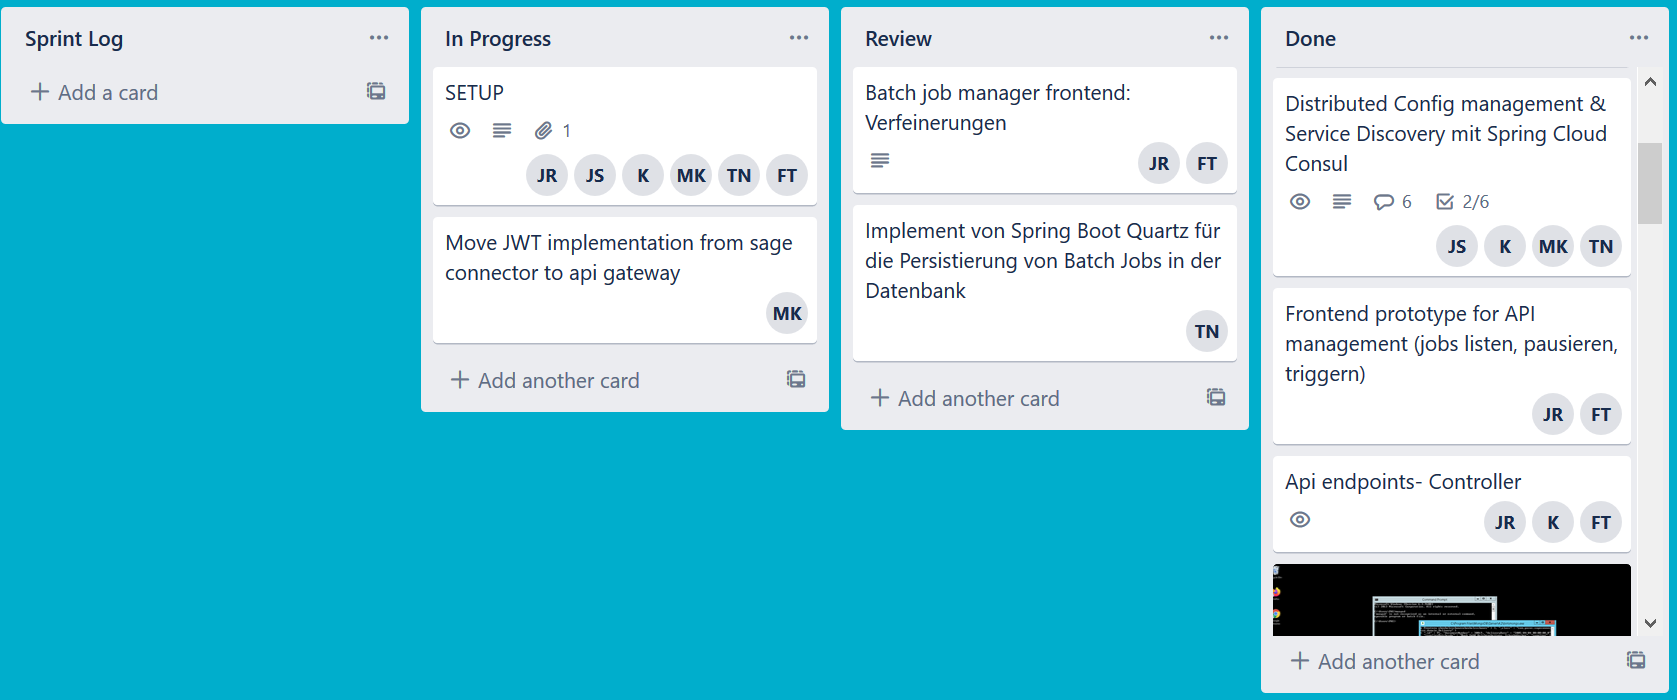
\includegraphics[width=15cm]{images/0x_organization/TrelloBoard.PNG}
\caption{Trello Board}
\label{fig:trello}
\end{figure}

\subsection*{\textbf{Implementierung}}
Für die gemeinsame Implementierung wurden Repositories in gitlab verwendet. Ein Vorteil den die Webanwendung gitlab bietet ist die Versionsverwaltung von Softwareprojekten. Durch die Implementierung in verschiedenen Branches konnten einzelne Aufgaben voneinander getrennt bearbeitet werden und abschließend in den Master Branch gepusht werden. Die einzelnen Arbeiten der Teammitglieder konnten über diesen Weg nicht nur geteilt, sondern auch nachvollzogen werden.

\subsection*{\textbf{Dokumentation}}
Um mit Statistance insbesondere die Rechercheergebnisse zu teilen, wurde Google Drive verwendet. In einem Studenten-Bereich von Statistance konnten alle Dokumente zur Recherche, wie zum Beispiel zu einzelnen Frameworks, Statistance zur Verfügung gestellt werden. Zur fortlaufenden Dokumentation von Meetings und Rücksprachen mit Statistance wurde ein Team Dokument in Google docs verwendet. Hier wurden von Projektstart bis Projektende jegliche Festlegungen, Treffen und sonstige wichtige Informationen festgehalten. Für den Abschlussbericht wurde Overleaf zur gemeinsamen Bearbeitung verwendet.


